\scanpage{66}
% block: gerbe class
\[
\handwritten{\xi\in}H^{\handwritten{2}}(k_{\mathrm{pl}},G)
\]
est la classe de la gerbe tannakienne qui définit $\handwritten{\unsure{\deleted{\mathcal{A}}\mathcal{M}|\deleted{\mathcal{M}}\mathcal{A}|\mathcal{M}}}$. Donc la connaissance du caractère numérique de $\handwritten{\mathcal{M}}$ équivaut à la donnée, en plus \unsure{du|de|da}\\ \hspace*{3cm}\deleted{\inserted{(qui implique déjà la donnée}}\\ groupe de t.m. $G$ sur $k$, des classes $u_{\unsure{\deleted{\illegible{1}}\handwritten{*}|\handwritten{\sigma}}}(\handwritten{\xi})$ pour tous les homomorphismes $u$ de $G$ dans des tores de la forme $\handwritten{\prod}_{Z/k}\underline{G}_m$, où $Z$ est une extension finie de $k$. \deleted{(}On vient de voir en effet que la donnée du caractère numérique permet de reconstituer ce qui précède. Pour voir l'inverse, notons que \deleted{si} le rang $\unsure{\deleted{d}n|\deleted{n}d}(\handwritten{\deleted{\unsure{\xi}}\sigma})$ de $M_{\handwritten{\sigma}}$ est déterminé par la formule
\[
n(\handwritten{\sigma})=\operatorname{card}(\handwritten{\sigma})\operatorname{\unsure{\deleted{d}o|\deleted{o}d}rd}(\handwritten{\xi_\sigma})
\]
(où $\operatorname{card}\handwritten{\sigma}$ est le cardinal de l'orbite $\handwritten{\sigma}$, $\operatorname{ord}(\handwritten{\xi_\sigma})$ est l'ordre de $\handwritten{\xi_\sigma}$ dans $\operatorname{Br}(Z_{\handwritten{\sigma}})$).

% block: determination question
La question de savoir si le caractère numérique détermine à équivalence de catégories tannakiennes près revient donc, pour $G$ fixé, à la question de savoir si un élément \deleted{de} $\handwritten{\xi\in}H^{\handwritten{2}}(k_{\mathrm{pl}},G_{\deleted{\times}})$ est connu quand on connait les $u_{\handwritten{*}}(\handwritten{\xi})$ pour $u:G\handwritten{\unsure{\mathrel{\begin{tikzpicture}[x=1cm,y=1cm,baseline=-.05cm]\draw[thin] (0,0)--(.5,0)--(.47,.12);\end{tikzpicture}}|\longrightarrow}}\underline{Z}^{\unsure{\times|x|\mathbb{x}|*}}$ comme dessus. \deleted{On va e\unsure{t|x|i}e\unsure{s}} C'est le cas pour $G$ diagonalisable \deleted{pro-dénombrable} (pro-dénombrable ?). On va examiner deux autres cas.

% block: example 1
\uline{Exemple} \unsure{$\mathbb{I}$|I|1}. $G$ est un tore de dimension 1, donc (s'il n'est trivial) tordu par une extension quadratique $Z$ de $k$. On a donc une suite exacte
\diagram{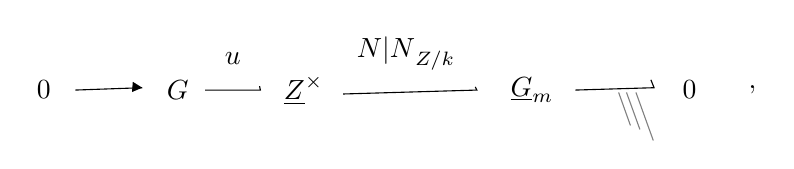
\begin{tikzpicture}[x=1cm,y=1cm]
\node at (0,0) {$0$};\node at (1.7,0) {$G$};\node at (3.3,0) {$\underline{Z}^{\times}$};\node at (6.2,0) {$\underline{G}_m$};\node at (8.2,0) {$0$};\node at (9,0) {$,$};
\draw[thin] (.4,0)--(1.25,.03);\fill (1.12,-.025)--(1.25,.03)--(1.13,.105)--cycle;
\draw[thin] (2.05,0)--(2.75,0)--(2.74,.05);\node at (2.4,.4) {$u$};
\draw[thin] (3.8,-.05)--(5.5,0)--(5.48,.04);\node at (4.6,.46) {$\unsure{\mathbb{N}|N}_{Z/k}$};
\draw[thin] (6.75,0)--(7.75,.03)--(7.71,.13);
\draw[thin,gray] (7.3,-.03)--(7.45,-.45);\draw[thin,gray] (7.4,-.03)--(7.57,-.5);\draw[thin,gray] (7.52,-.03)--(7.74,-.64);
\end{tikzpicture}}
d'où on conclut, par la suite exacte de cohomologie et le th. 90 que $\operatorname{Ker}(u:H^{\handwritten{2}}(k,G)\handwritten{\longrightarrow}H^{\handwritten{2}}(\unsure{\deleted{i}k|\deleted{k}i},\underline{Z}^{\times}))$ est nul. Donc dans le cas envisagé, le caractère numérique détermine $\handwritten{\mathcal{M}}$ à équivalence près.

% block: cancelled example 2
\deleted{\uline{Exemple} 2. Gardons \deleted{l\unsure{'|i|t}e} $G$ comme dessus, soit $n$ un entier $\quad2$, et soit $G'=\operatorname{Ker}n.\operatorname{id}_G$. La suite exacte}
\diagram{\begin{tikzcd}[ampersand replacement=\&]
\deleted{0} \& \deleted{G'} \& \deleted{G} \arrow[r,phantom,"\deleted{n}"] \& \deleted{G} \& \deleted{0}
\end{tikzcd}}
\deleted{et le résultat précédent montre que l'ensemble des classes de}
\figure{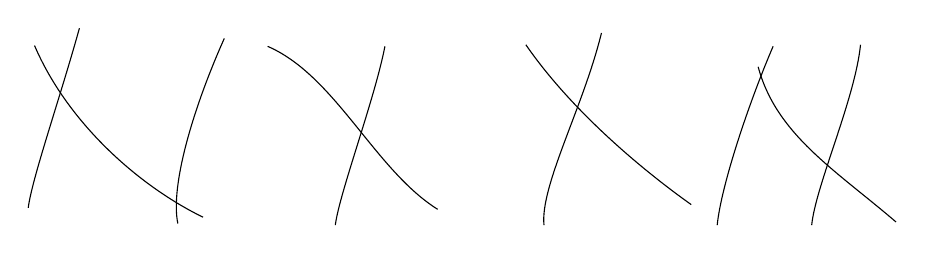
\begin{tikzpicture}[x=1cm,y=1cm]
\draw[thin] (.95,2.4).. controls (.7,1.5) and (.35,.5)..(.3,.12);
\draw[thin] (.38,2.18).. controls (.8,1.2) and (1.7,.4)..(2.52,0);
\draw[thin] (2.79,2.27).. controls (2.4,1.4) and (2.1,.4)..(2.2,-.08);
\draw[thin] (3.34,2.17).. controls (4.2,1.8) and (4.7,.6)..(5.5,.1);
\draw[thin] (4.83,2.17).. controls (4.7,1.5) and (4.25,.3)..(4.2,-.1);
\draw[thin] (6.62,2.19).. controls (7.2,1.35) and (8.1,.6)..(8.72,.16);
\draw[thin] (7.58,2.34).. controls (7.35,1.4) and (6.8,.4)..(6.85,-.1);
\draw[thin] (9.76,2.17).. controls (9.45,1.45) and (9.1,.4)..(9.05,-.1);
\draw[thin] (9.57,1.91).. controls (9.8,1.05) and (10.55,.6)..(11.32,-.06);
\draw[thin] (10.87,2.19).. controls (10.8,1.5) and (10.3,.4)..(10.25,-.1);
\end{tikzpicture}}
% archive sheet number: 65
